\chapter{Resultados Parciais}\label{resultados}

\section{Testes em imagens estáticas} \label{testesEstaticas}

Os primeiros testes aplicados no programa foram feitos com imagens estáticas ao invés de imagens de vídeo. O propósito destes testes era verificar a eficácia do algoritmo de diferenciação de fundos detalhado na seção \ref{diferencasFundos}. Cada imagem estática fazia o papel de uma imagem de fundo que teria sido extraída de um vídeo da câmera no estacionamento. As imagens para os primeiros testes foram obtidas com o auxílio de um \textit{drone} de controle remoto que fez fotografias aéreas do estacionamento próximo aos prédios PAT e PJC no campus da Universidade de Brasília. A fim de simular melhor a imagem que seria obtida por uma câmera instalada em um poste no estacionamento, um programa de edição de imagens foi utilizado para recortar pedaços da imagem com um nível maior de aproximação. Essas foram as imagens utilizadas para os testes.

A primeira etapa dessa bateria de testes foi testar o caso mais simples de todos: comparar uma imagem de fundo com a imagem do estacionamento completamente desocupado. Através de manipulação de imagens, foram compostas diversas imagens com carros de cores diferentes, estacionados em várias combinações distintas de vagas. Cada imagem é comparada a imagem da seção de estacionamento correspondente com todas as vagas desocupadas. Aqui, uma diferença entre as duas imagens que esteja em uma região que se sabe que é uma vaga sempre representa um carro que passou a ocupar aquela vaga. Uma terceira imagem mostra através de círculos coloridos quais vagas estão ocupadas na imagem de teste.  Nessa etapa de testes, o programa obteve uma taxa de acerto de 100\%. A figura \ref{ComparacaoFundoVazioFig} mostra alguns resultados desses testes.

O bom funcionamento nesse caso simples é de grande importância. Se o programa for inicializado com o estacionamento vazio, a primeira comparação de fundo será dessa maneira. Se o algoritmo acerta quais vagas estão ocupadas, ele agora está munido da informação completa dos estados das vagas. A partir desse momento, é possível interpretar de forma mais simples as diferenças na imagens de fundo obtidas no vídeo. Uma diferença significativa sobre uma região de vaga livre, significa que a vaga foi ocupada. Se a vaga estava ocupada, ela foi liberada entre uma verificação e outra. Assim, o algoritmo consegue indicar o estado das vagas com uma taxa muito alta de acerto através de operações simples, desde que o estado inicial seja conhecido.

\begin{figure}
 \centering
\begin{subfigure}{.5\textwidth}
  \centering
  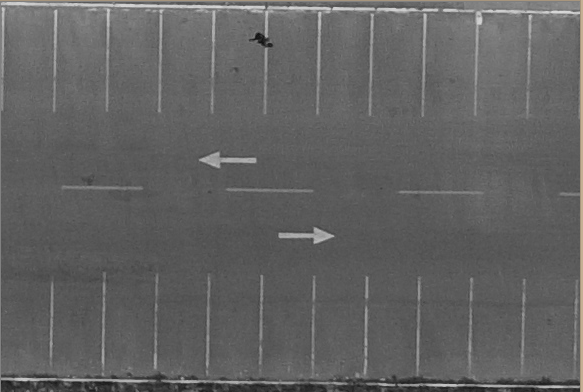
\includegraphics[width=.8\linewidth]{Vazio}
  \caption{}
  \label{ComparacaoFundoVazioFig:sfig1}
\end{subfigure}\

\begin{subfigure}{.5\textwidth}
  \centering
  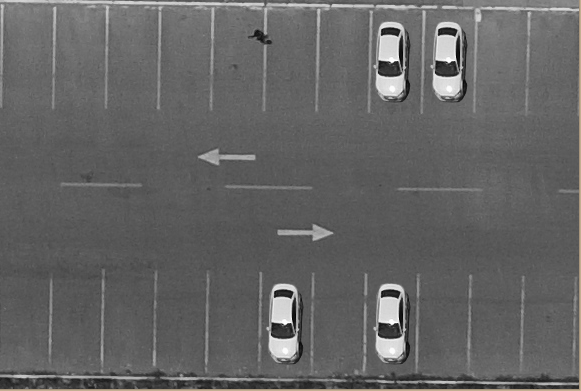
\includegraphics[width=.5\linewidth]{4Carros}
  \caption{}
  \label{ComparacaoFundoVazioFig:sfig2}
\end{subfigure}%
\begin{subfigure}{.5\textwidth}
  \centering
  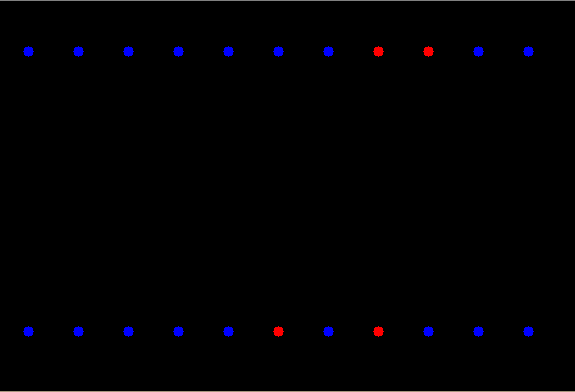
\includegraphics[width=.5\linewidth]{Indicacao4Carros}
  \caption{}
  \label{ComparacaoFundoVazioFig:sfig3}
\end{subfigure}

\begin{subfigure}{.5\textwidth}
  \centering
  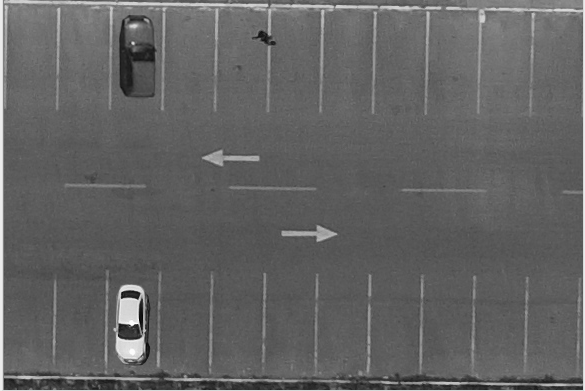
\includegraphics[width=.5\linewidth]{2Carros}
  \caption{}
  \label{ComparacaoFundoVazioFig:sfig4}
\end{subfigure}%
\begin{subfigure}{.5\textwidth}
  \centering
  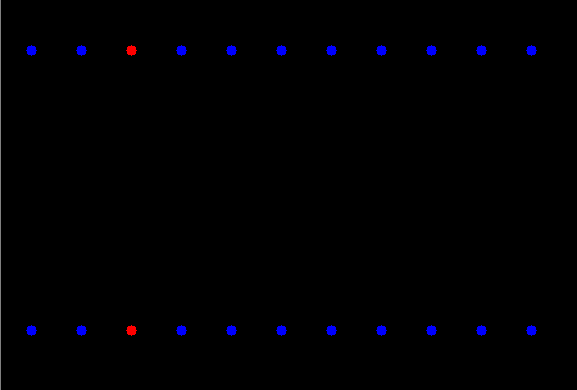
\includegraphics[width=.5\linewidth]{Indicacao2Carros}
  \caption{}
  \label{ComparacaoFundoVazioFig:sfig5}
\end{subfigure}



\caption{(a) O estacionamento vazio; (b) Quatro carros estacionados; (c) As indicações de ocupação das vagas em (b); (d) Dois carros estacionados; (e) As indicações dos estados das vagas em (d)}
\label{ComparacaoFundoVazioFig}
\end{figure}

Infelizmente, nem sempre se conhece o estado inicial do vetor de vagas quando o algoritmo começa a executar. Ele pode ter sido iniciado sobre um estacionamento que não estava completamente vazio ou a câmera ter sido desligado durante sua execução. Nesse caso o programa precisa ser capaz de determinar o estado das vagas a partir de uma determinada imagem do vídeo, normalmente uma imagem de fundo para a partir daí poder utilizá-lo para as avaliações futuras. Além disso, é preciso utilizar as técnicas apresentadas nas seções \ref{identificacaoFundo} e \ref{verificaoObjetosFundo} para evitar falsos positivos.


Por causa disso, a segunda etapa de testes consiste na comparação de duas imagens de fundo de momentos diferentes. O programa deve então ser capaz de utilizar as técnicas apresentadas e determinar corretamente o estado de ocupação das vagas sem se utilizar do conhecimento prévio do estado anterior. Para realizar essa tarefa, o programa verifica novamente as diferenças nas vagas. Nas regiões onde houve diferença, como aquela indicadas na figura \ref{regioesDiferencaTesteFig} o programa faz a comparação de histograma com o estado anterior para determinar se o movimento foi de chegada ou saída de um veículo. Se utilizando dessa comparação o programa atualiza o vetor dos estados das vagas. Os estados das vagas onde não houve diferença pode ser determinado por classificação de objetos ou também por uma comparação de histogramas, basta comparar o histograma com o de controle ou com o de uma vaga que acabou de ser desocupada.


\begin{figure}
 \centering
 \begin{subfigure}{.5\textwidth}
  \centering
  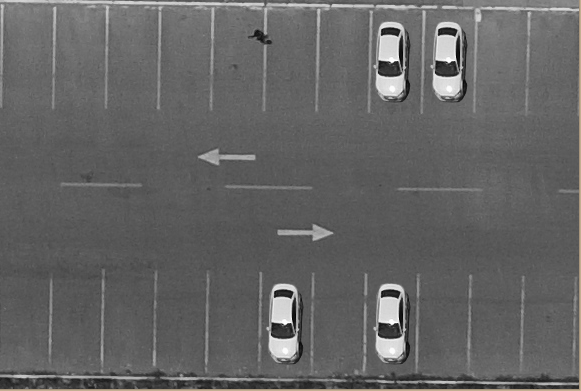
\includegraphics[width=.5\linewidth]{4Carros}
  \caption{}
  \label{regioesDiferencaTesteFig:sfig1}
\end{subfigure}%
\begin{subfigure}{.5\textwidth}
  \centering
  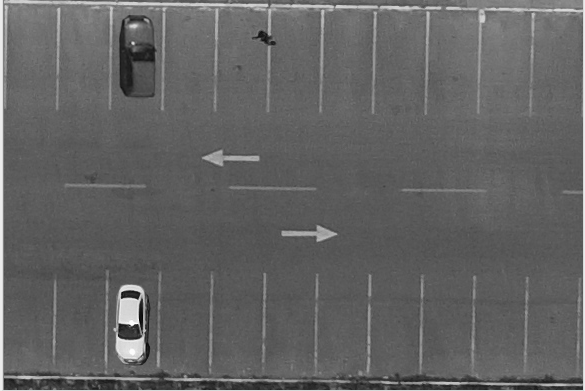
\includegraphics[width=.5\linewidth]{2Carros}
  \caption{}
  \label{regioesDiferencaTesteFig:sfig2}
\end{subfigure}

 \begin{subfigure}{.5\textwidth}
  \centering
  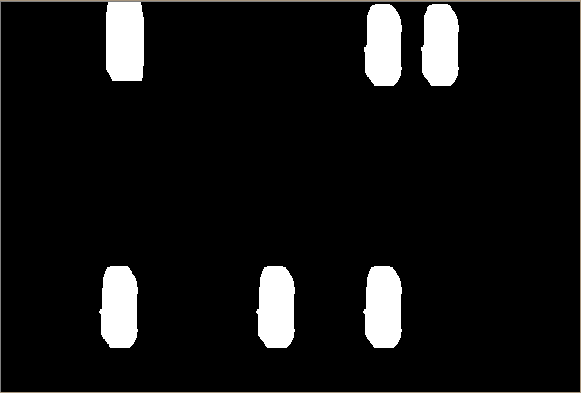
\includegraphics[width=.8\linewidth]{Diferenca4-2Carros}
  \caption{}
  \label{regioesDiferencaTesteFig:sfig3}
\end{subfigure}%


\caption{(a) Quatro carros estacionados; (b) Dois carros estacionados; (c) As manchas que indicam aonde houve diferença entre as duas imagens.}
\label{regioesDiferencaTesteFig}
\end{figure}

Apesar das indicações de diferença parecerem muito precisas, nenhum dos métodos de comparação de histograma apresentados na subseção \ref{comparacaoHistogramas} foi suficiente para que o programa tivesse uma taxa de acerto satisfatória até agora, mas ela tem aumentado a cada nova versão do programa. Esse algoritmo vai continuar a ser aprimorado para as próximas etapas do trabalho. A tabela \ref{tabelaDiferencasHistogramas} mostra os valores obtidos pela diferença $\chi^2$ e pelo cálculo de intersecção das vagas com o histograma de controle, e a figura \ref{histogramasRegioesPequenas} mostra os histogramas de cada uma delas e o histograma de controle.

Analisando essa tabela e as imagens dos histogramas, pode-se perceber que os valores obtidos não são suficiente para se determinar um limiar de semelhança com nenhuma das duas técnicas ainda. Imagens semelhantes estão apresentando um distância maior do que o esperado. O maior fator impeditivo é a grande disparidade entre os valores das vagas 4 e 5, que estão ambas vazias e deveriam mostrar valores similares quando comparadas ao histograma de controle.


\begin{figure}
 \centering
 \begin{subfigure}{\textwidth}
  \centering
  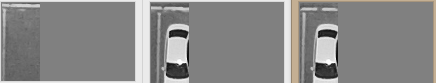
\includegraphics[width=\linewidth]{RegioesPequenas1}
  \caption{}
  \label{regioesPequenasTesteFig:sfig1}
\end{subfigure}%

\begin{subfigure}{\textwidth}
  \centering
  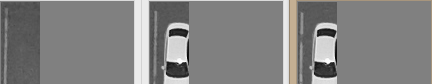
\includegraphics[width=\linewidth]{RegioesPequenas2}
  \caption{}
  \label{regioesPequenasTesteFig:sfig2}
\end{subfigure}


\caption{As diferentes regiões da imagem de fundo que são analisadas no caso apresentado na figura \ref{regioesDiferencaTesteFig}. Na parte superior da esquerda para a direita: vagas 5, 15 e 17. Na parte inferior vagas 4, 10 e 14.}
\label{regioesPequenasTesteFig}
\end{figure}


\begin{figure}
 \centering
  \begin{subfigure}{.3\textwidth}
  \centering
  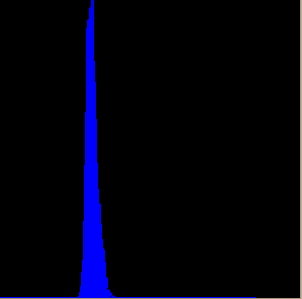
\includegraphics[width=.8\linewidth]{HistogramaControle}
  \caption{}
  \label{histogramasRegioesPequenasFig:sfig1}
\end{subfigure}%


 \begin{subfigure}{.8\textwidth}
  \centering
  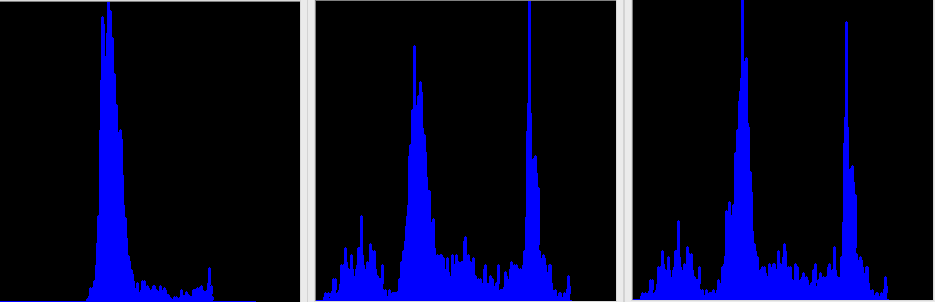
\includegraphics[width=.5\linewidth]{histogramasTesteSuperior}
  \caption{}
  \label{histogramasRegioesPequenasFig:sfig1}
\end{subfigure}%

\begin{subfigure}{.8\textwidth}
  \centering
  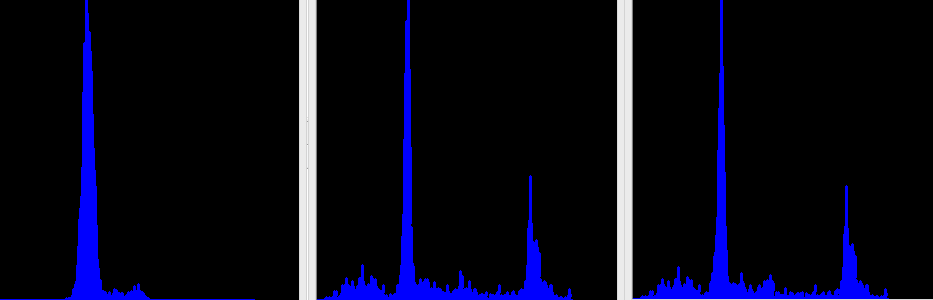
\includegraphics[width=.5\linewidth]{histogramasTesteInferior}
  \caption{}
  \label{histogramasRegioesPequenasFig:sfig2}
\end{subfigure}


\caption{(a)O histograma de controle; (b) Os histogramas das imagens apresentadas em  \ref{regioesPequenasTesteFig:sfig1}; (c) Os histogramas das imagens apresentadas em  \ref{regioesPequenasTesteFig:sfig2};}
\label{histogramasRegioesPequenasFig}
\end{figure}




\begin{table}
\centering
 \begin{tabular}{||c c c||}
 \hline
 Vaga & $\chi^2$ & Intersecção \\ [0.5ex]
 \hline\hline
 4 & 2371.72 & 2442.04 \\
 \hline
 5 & 189588 & 476.993 \\
 \hline
 10 & 15373.5 & 1428.9 \\
 \hline
 14& 8747.21 & 1506.91 \\
 \hline
 15 & 33113.5 & 809.946 \\
 \hline
 17 & 113295 & 474.473 \\ [1ex]
 \hline
\end{tabular}

\caption{A tabela com os valores obtidos pelas duas técnicas de comparação de histograma utilizadas}
\label{tabelaDiferencasHistogramas}
\end{table}




Se acredita que a melhor solução para atingir uma taxa de acerto satisfatória é melhorar a técnica que o programa se utiliza para determinar a região da imagem de fundo original a ser analisada a partir da imagem de diferença \ref{regioesDiferencaTesteFig:sfig3}.Atualmente, o programa determina os contornos da imagem e calcula a partir deles o menor retângulo inclinado $R$ que os contém e em seguida obtém o retângulo aonde $R$ está inscrito. Esse segundo retângulo determina a região da imagem de fundo a ser analisada para cada vaga. Na figura \ref{regioesPequenasTesteFig} pode-se observar que essa técnica obtém regiões que não são completamente precisas. Essa falha atrapalha a medição e gera resultados indesejados. A solução que está sendo explorada envolve adaptar a região contida em $R$ para que ela apareça sem inclinação em uma outra imagem, facilitando a análise e aumentando a precisão dos resultados.

Outra solução que possivelmente aumentará a precisão dos resultados é converter cada fração da imagem de fundo que está sendo analisada para o formato HSV, que é a representação mais natural da visualização de imagens, e fazer a comparação de histogramas normalizados do canal H dessas imagens. Essa mudança é a próxima etapa do trabalho e se acredita que pode ser um ponto crucial na sua implementação, uma vez que aumentar a taxa de acerto nessa etapa permite avançar para a próxima etapa de implementação.

\section{Primeiros testes em vídeos}\label{testesVideos}

A outra parcela de testes que já foi executada sobre o programa utilizou vídeos adquiridos \textit{online}. Foram utilizados vídeos da internet por causa da dificuldade de se obter filmagens úteis nesse momento da execução do trabalho. O propósito dessa etapa de testes era avaliar o funcionamento do algoritmo de geração dinâmica de \textit{background} exposto na seção \ref{geracaoFundo} e experimentar com o algoritmo de rastreamento descrito na seção \ref{rastreamentoVeiculos}. Por causa da natureza e do propósito dos testes, algumas das filmagens utilizadas nesse momento não são de estacionamentos, uma vez que nesse etapa não se fazia totalmente necessário que as imagens analisadas fossem completamente coerentes com aquelas que virão a ser analisadas pelo programa no futuro. Em um momento posterior da implementação do trabalho, pretende-se gerar animações através das imagens estáticas utilizadas na seção \ref{testesEstaticas} e filmagens em um modelo em escala de um estacionamento real, para que possam ser feitos testes provisórios antes da etapa de validação do algoritmo.

\subsection{Testes de geração de fundo} \label{testesFundo}

Foram feitos testes do algoritmo de geração dinâmica de fundo (\ref{geracaoFundo}) em um vídeo de uma câmera de um estacionamento e em uma série de vídeos de câmeras de segurança de vias de trânsito obtidos através da internet. Para satisfazer os testes, o algortimo deveria cumprir uma série de condições:
    \begin{itemize}
      \item No vídeo resultante do sistema os objetos em movimento no vídeo original deveriam estar completamente invisíveis ao olho humano.
      \item As regiões de diferença obtidas deveriam estar suficientemente próximas dos objetos em movimento no vídeo original.
      \item O algoritmo deveria ser capaz de integrar objetos que entraram na cena e pararam de se mover ao fundo.
      \item Também deve ser capaz de perceber que objetos antes integrados ao fundo passaram a se mover.
      \item Não deve fazer operações sobre diferenças insignificantes entre dois quadros de vídeo.
    \end{itemize}

A primeira condição apresentada, obviamente, irrelevante para o sistema de computador, mas é um bom indicador para os desenvolvedores do funcionamento do algoritmo e está fortemente ligada ao cumprimento da segundo condição, tendo a vantagem de ser muito mais fácil e intuitiva de se verificar. As condições sobre a mudança de estado de objetos para o fundo são também de fácil verificação, mas são de extrema importância para o trabalho. Se o algoritmo não for capaz de cumprir essas duas condições, ele não é adequado para o sistema que esse projeto visa desenvolver. A última condição é de mais difícil verificação, mas por sorte é também a menos relevante delas, uma vez que existe um mecanismo redundante para eliminiação de regiões de diferença insignificante na etapa de subtração de fundos descrita na seção \ref{testesEstaticas}.

No geral, o algoritmo se mostrou muito capaz de cumprir todas as condições. Apesar de haverem momentos onde o resultado não foi totalmente perfeito, o programa teve desempenho satisfatório sobre as regiões relevantes em todos os vídeos de teste. Durante os testes, percebeu-se que o algoritmo funcionava muito melhor quando tratava de veículos em velocidades maiores e cores mais claras. Isso era de se esperar pela implementação do algoritmo. Objetos que se movem mais rapidamente geram diferenças quadro-a-quadro maiores e por isso a região obtida aonde o programa assume que existe um veículo é mais precisa. Como consequência dessa característica, ao olho humano, veículos que estão desacelerando passam a aparecer gradualmente na vídeo de fundo, a medida que pedaços dele passam a se mover muito pouco para que a diferença seja siginificativa. Isso não interfere na execução do problema, por causa da natureza periódica da subtração entre fundos. Uma escolha correta do intervalo de tempo para subtração e pesos das imagems do quadro inicial e fundo anterior no momento de geração amenizam ainda mais esse aparecimento gradual. Quando um objeto passava a se movimentar o algoritmo sempre era capaz de perceber essa mudança imediatamente, porém, por causa da natureza da geração do fundo, o desaparecimento é gradual. Novamente, um ajuste de parâmetros traz esse problema para níveis aceitávies. A figura \ref{figTestesFundos} demonstram alguns resultados.

\begin{figure}
 \centering
  \begin{subfigure}{.6\textwidth}
  \centering
  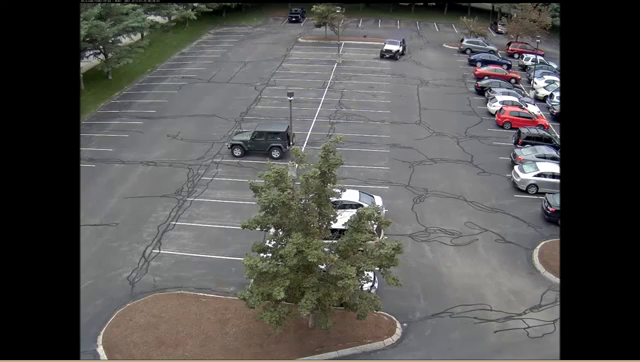
\includegraphics[width=.5\linewidth]{Video}
  \caption{}
  \label{figTestesFundos:sfig1}
\end{subfigure}%
 \begin{subfigure}{.6\textwidth}
  \centering
  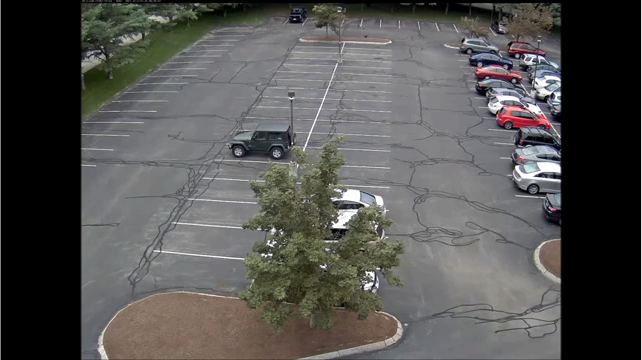
\includegraphics[width=.5\linewidth]{Fundo}
  \caption{}
  \label{figTestesFundos:sfig2}
\end{subfigure}

\begin{subfigure}{.6\textwidth}
  \centering
  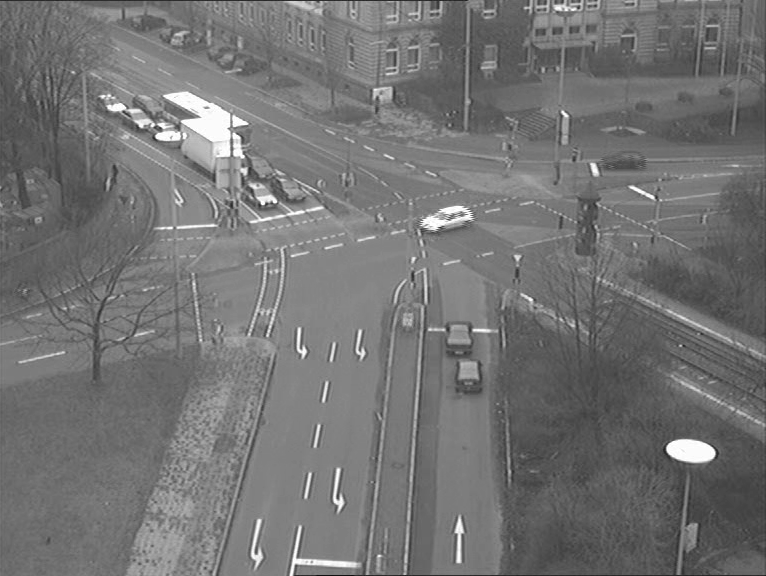
\includegraphics[width=.5\linewidth]{Quadro1}
  \caption{}
  \label{figTestesFundos:sfig3}
\end{subfigure}%
\begin{subfigure}{.6\textwidth}
  \centering
  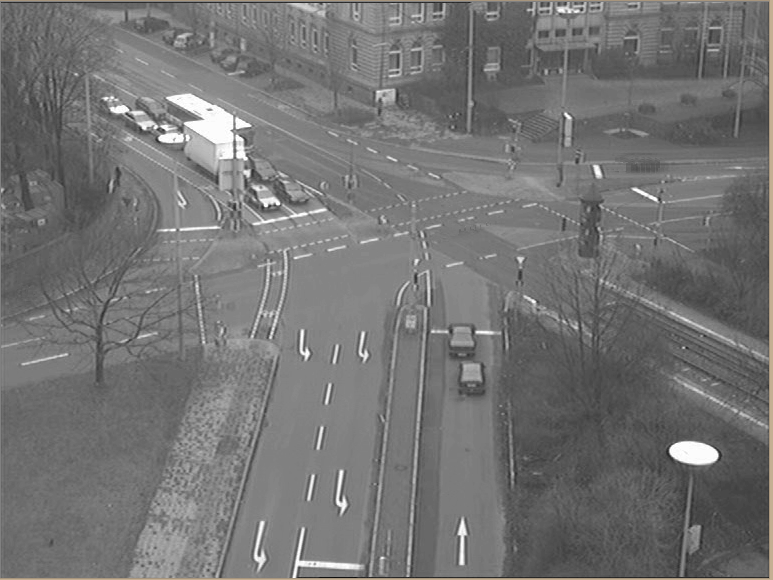
\includegraphics[width=.5\linewidth]{Fundo1}
  \caption{}
  \label{figTestesFundos:sfig4}
\end{subfigure}


\caption{(a) e (b) um quadro do vídeo de um estacionamento e o fundo correspondente; (c) e (d) um quadro de um dos vídeos de tráfego e o seu fundo correspondente.}
\label{figTestesFundos}
\end{figure}


Para a verificação da última condição a saída do algoritmo foi modificada. Ao invés de retornar um vídeo contendo apenas a imagem do fundo, para esses testes o algoritmo mostrava na tela um vídeo de um fundo completamente preto, exceto pelas regiões de \textit{foreground}. Dessa forma era possível avaliar quais regiões estavam sendo consideradas como suficientemente diferentes para o algoritmo. Esses testes mostraram que em imagens com pouco ou nenhum ruído, o mecanismo apresentado de eliminição de pequenas regiões funciona com 100\% de satisfação. Apenas as regiões com objetos em movimento eram mostradas na saída de vídeo. Em imagens muito ruidosas porém, percebeu-se que é necessário um tratamento prévio, a fim de eliminar o ruído presente. É preciso então avaliar métodos de remoção de ruído de imagens e determinar um que seja capaz de eliminar as impurezas indesejadas sem interferir na detecção dos objetos em movimento. A figura \ref{testeSegmentacaoFig} mostra a saída dessa forma do quadro mostrado na figura \ref{figTestesFundos:sfig3}. Nela pode-se perceber um pequeno erro causado por ruído e falhas na segmentação do carro preto no canto superior direito da tela.

\begin{figure}
 \centering
  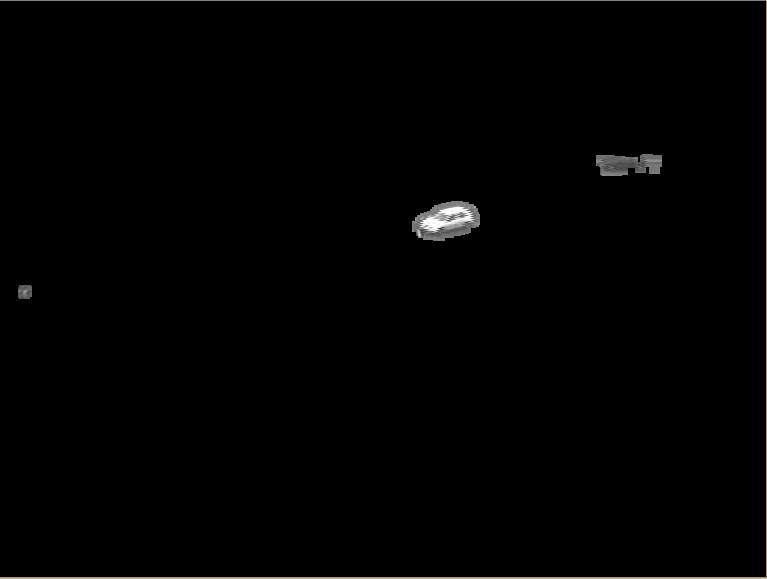
\includegraphics[width=.5\textwidth]{Seg1}  
    \caption{A segmentação do algoritmo de geração de fundo quadro na figura \ref{figTestesFundos:sfig3}.}
\label{testeSegmentacaoFig}
\end{figure}

Ao fim destes testes, se concluiu que o algoritmo da forma como está implementado agora cumpre satisfatoriamente as necessidades impostas pelo programa e é completamente adequado para as tarefas exigidas para o seu funcionamento. O algoritmo mostrou resultados excelentes em geração de fundo para veículos em velocidade moderada e se movendo continuamente. Ainda é também capaz de integrar corretamente ao fundo da imagem qualquer objeto que interrompa seu movimento por tempo suficiente. Acredita-se ainda que esse algoritmo seja útil em diversos outros trabalhos. Por exemplo, com poucos ajustes o algoritmo seria perfeitamente capaz de detectar veículos que estejam se movimento sobre uma rodovia e poderia ser usado em programa de análise de fluxo de tráfego.

\subsection{Testes do sistema de rastreamento} \label{testesRastreamento}

Para os testes do sistema descrito na seção \ref{rastreamentoVeiculos}, foi usado apenas o vídeo que contém a filmagem do movimento em um estacionamento. Vídeos de câmera de tráfego em ruas tornavam a análise muito difícil em razão do elevado número de rastros gerados. Obviamente, mais testes serão elaborados posteriormente, quando filmagens mais adequadas forem obtidas.

As análises executadas sobre o resultado desse sistema forem principalmente visuais, de forma que o resultado era analisado através de observação humana da imagem resultante do processo. A preocupação principal nesses testes era a corretude das posições dos círculos desenhados no rastro e a identificação correta da posição relativa entre o início e o fim dos rastros e o interior de vagas, verificado através de informação exibida na saída padrão do computador pelo programa.

É de extrema importância que o programa seja capaz de identificar que um rastro representa um trajeto que teve início fora de uma vaga e final no seu interior. Não apenas isso, é crucial que ele não acuse falsos positivos no caso de um veículo passar rapidamente por dentro de uma região que representa uma vaga mas não estacionar. Essa detecção é parte do mecanismo de verificação do estado das vagas, juntamente com a subtração dos fundos em momentos distintos.

Os testes sobre o vídeo em questão mostraram que o sistema é totalmente capaz de detectar e desenhar corretamente na tela de saída um rastro que representa o trajeto de veículos em movimento no estacionamento. Além disso, as condições e parâmetros para decidir se um contorno de diferença faz parte do trajeto se mostraram suficientes e corretos. Também se observou uma taxa total de acertos na posição relativa entre os pontos inicias e finais e o interior das vagas. Porém, o programa apresentou alguns defeitos nessa etapa. Diferenças pequenas na imagem, causadas por ruído ou movimentos pequenos em uma região geravam rastros muito curtos, algumas vezes com um só ponto. Apesas desses rastros não representarem um problema muito siginificante nesse momento, porque na grande maioria dos casos vão se iniciar e terminar em ponto quase iguais e não vão acusar que houve movimento para dentro ou fora de uma vaga, reconhece-se que eles são indesejados e a aparição deles não é uma situação ideal e é potencialmente perigosa para o bom funcionamento do programa. A figura \ref{testesRastrosFig} mostra dois rastros em um vídeo. Na figura os pequenos rastros problemáticos são visíveis na região da árvore.

\begin{figure}
 \centering
  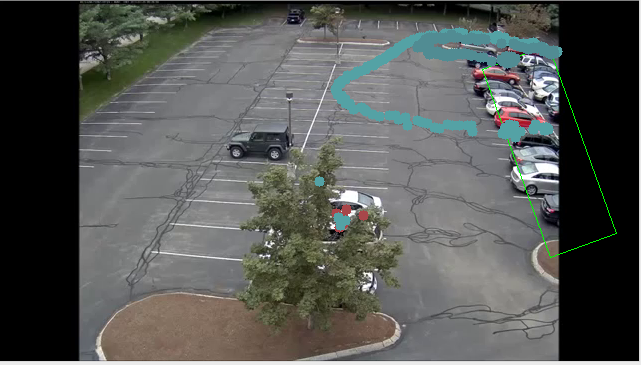
\includegraphics[width=.5\textwidth]{2Rastros}
    \caption{O rastro de dois carros em um vídeo de um estacionamento.}
\label{testesRastrosFig}
\end{figure}

Concluiu-se então que é preciso refinamento nesse componente do programa. Apesar do algoritmo utilisado atualmente ser capaz de mostrar visualmente um rastro de um veículo com bastante precisão, ele apresenta diversos riscos para falsos positivos que não devem ser desconsiderados na implementação final do programa. Métodos diferentes de rastreamento e outras alternativas já estão sendo estudados para implementação.


